
\chapter{Suffix-tracking sets -- obtaining DSA from DFA}
\label{sec:suffix-tracking-sets}

The previous chapter formally defined Deterministic Suffix-reading Automata and demonstrated their potential for providing highly succinct representations of regular languages. However, a model's practical utility hinges on our ability to systematically construct it for a given language. This chapter addresses that crucial problem: how does one derive a correct and concise DSA from a standard representation like a DFA?

Our approach is centered on a form of abstraction, or state suppression. The core intuition is to "downsample" a given DFA by selecting a subset of its states to serve as the primary "macro-states" of the new DSA, while the paths between them become the new, string-based transitions. This general strategy is not new; a similar state-suppression method exists for generating Deterministic Generalized Automata~\cite{giammarresi1999deterministic}. However, the challenge is significantly greater for DSAs. The sophisticated, non-local semantics of suffix-reading mean that the suppressed states and the paths through them must collectively behave as a single, consistent suffix-matcher. Naively collapsing paths without respecting this underlying semantic requirement can easily alter the accepted language.

For the derivation to be sound, the collection of paths that will become the new DSA transitions must satisfy stringent consistency requirements. An analogy can be drawn to ensuring a complex electronic circuit is functional: it is not enough for the individual wires to be well-made; they must also be connected correctly at their terminals to avoid ambiguity and short-circuits. Our derivation procedure rests on two such conditions.

First, we must ensure that the paths are \textbf{internally consistent}. This is the role of the `suffix-compatibility' condition. It guarantees that as we trace a path through the suppressed part of the DFA, the logic of suffix-matching is maintained correctly at every single step. This is akin to checking that each wire in the circuit functions correctly along its entire length, faithfully transmitting signals.

Second, we must ensure the paths are consistent with each other at their \textbf{endpoints}—the selected macro-states. This is the purpose of the `well-formedness' condition. It prevents ambiguity by forbidding situations where a path leading to a chosen macro-state could be mistaken for part of a different path leading to a suppressed state. This is analogous to checking that all wires are connected to the correct terminals in the circuit, ensuring that signals arrive at their intended destinations without interference.

This chapter will formalize these ideas, culminating in the definition of a `suffix-tracking set': a set of states that satisfies both of these conditions. The main theorem will then prove that any DSA derived from such a set is guaranteed to be sound and language-equivalent to the source DFA.

%marker
\vspace{0.25cm}

For DGAs, a
method to derive smaller DGAs by suppressing states was 
recalled in Section~\ref{sec:preliminaries}. Our goal is to
investigate a similar procedure for DSAs. The DSA model creates
new challenges. Suppressing states may not always lead to
smaller automata (in total
size). Figure~\ref{fig:minim-challenges-suppr-states} illustrates an
example where suppressing states leads to an exponentially larger
automaton, due to the exponentially many
paths created. But, suppressing states may sometimes
indeed be useful: in Figure~\ref{fig:suppressing-states-reduces-size},
the DFA on the left is performing a string matching to deduce the
pattern $ab$. On seeing $ab$, it accepts. Any extension is
rejected. This is succinctly captured by the DSA on the right. Notice
that the DSA is obtained by suppressing states $q_1$ and $q_3$. So,
suppressing states may sometimes be useful and sometimes not. In~\cite{giammarresi1999deterministic}, the focus was on
getting a DGA with minimal number of states, and hence suppressing
states was always useful.

More importantly, when can we suppress states? DGAs cannot ``ignore''
parts of the word. This in particular leads to the requirement that a
state with a self-loop cannot be suppressed. DSAs have a more
sophisticated transition semantics. Therefore, the procedure to
suppress states is not as simple. This is the subject of this
section. We deviate from the DGA setting in two ways:  we will select a subset of good states from which we can
construct a DSA (essentially, this means the rest of the states are
suppressed); secondly, our starting point will be complete DFA, on
which we make the choice of states (in DGAs, one could start
with any DGA and suppress states). Our procedure can be broken down
into two steps: (1) Start from a complete DFA, select a subset of states and
    build an induced DSA by connecting states using
    acyclic paths between them; (2) Remove some redundant
    transitions.


\begin{figure}
  \centering
  
    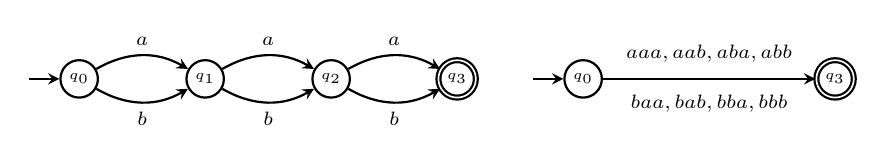
\begin{tikzpicture}[state/.style={circle, draw, thick, inner sep =
      2pt}, scale=0.8]
    \begin{scope}[every node/.style={state}]
      \node (0) at (0,0) {\tiny $q_0$};
      \node (1) at (2,0) {\tiny $q_1$};
      \node (2) at (4,0)  {\tiny $q_2$};
      \node [double] (3) at (6,0) {\tiny $q_3$};
    \end{scope}
    \begin{scope}[->, >=stealth, thick]
      \draw (-0.8,0) to (0);
      \draw (0) to [bend left] node [above] {\scriptsize $a$} (1); 
      \draw (0) to [bend right] node [below] {\scriptsize $b$} (1);
       \draw (1) to [bend left] node [above] {\scriptsize $a$} (2); 
       \draw (1) to [bend right] node [below] {\scriptsize $b$} (2);
        \draw (2) to [bend left] node [above] {\scriptsize $a$} (3); 
      \draw (2) to [bend right] node [below] {\scriptsize $b$} (3);
    \end{scope}

    \begin{scope}[xshift=8cm]
       \begin{scope}[every node/.style={state}]
      \node (0) at (0,0) {\tiny $q_0$};
      \node [double] (3) at (4,0) {\tiny $q_3$};
    \end{scope}

    \begin{scope}[->, >=stealth, thick]
      \draw (-0.8, 0) to (0);
      \draw (0) to (3);
    \end{scope}

    \node at (2, 0.4) {\scriptsize $aaa, aab, aba, abb$};
    \node at (2, -0.4) {\scriptsize $baa, bab, bba, bbb$};
    
    \end{scope}
  \end{tikzpicture}
  \caption{Suppressing states can add exponentially many labels and
    increase total size.}
  \label{fig:minim-challenges-suppr-states}
\end{figure}

\begin{figure}
  \centering
  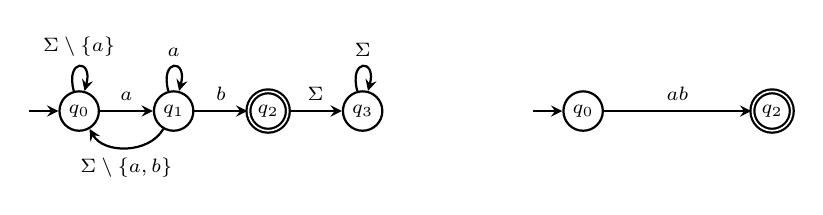
\begin{tikzpicture}[state/.style={circle, draw, thick, inner sep =
      2pt}, scale=0.8]
    \begin{scope}[every node/.style={state}]
      \node (0) at (0,0) {\scriptsize $q_0$};
      \node (1) at (1.5,0) {\scriptsize $q_1$};
      \node [double] (2) at (3,0) {\scriptsize $q_2$};
      \node (3) at (4.5,0) {\scriptsize $q_3$};
    \end{scope}
    \begin{scope}[->,>=stealth, thick, auto]
      \draw (-0.8, 0) to (0);
      \draw (0) to [loop above] node {\scriptsize $\Sigma
        \setminus \{a\}$} (0);
      \draw (0) to node {\scriptsize $a$} (1);
      \draw (1) to [bend left = 60] node [below] {\scriptsize $\Sigma
        \setminus \{a, b\}$} (0);
      \draw (1) to [loop above] node {\scriptsize $a$} (1);
      \draw (1) to node {\scriptsize $b$} (2);
      \draw (2) to node {\scriptsize $\Sigma$} (3);
      \draw (3) to [loop above] node {\scriptsize $\Sigma$} (3);
    
    \end{scope}

    \begin{scope}[xshift=8cm]
      \begin{scope}[every node/.style={state}]
        \node (0) at (0,0) {\scriptsize $q_0$};
        \node [double] (2) at (3,0) {\scriptsize $q_2$};
      \end{scope}
      \begin{scope}[->,>=stealth, thick, auto]
        \draw (-0.8, 0) to (0);
        \draw (0) to node {\scriptsize $ab$} (2);
      \end{scope}
    \end{scope}
  \end{tikzpicture}
  \caption{Suppressing states can sometimes reduce total size}
  \label{fig:suppressing-states-reduces-size}
\end{figure}

\paragraph{Building an induced DSA}

We start with an illustrative example. Consider DFA $M$ in
Figure~\ref{fig:induced-eqv}. 
The DSA on the right of the figure shows such an induced DSA obtained
by marking states $\{q_0, q_2\}$ and connecting them using simple
paths. Notice that the language of the induced DSA and the original
DFA are same in this case. Intuitively, all words that end with an $a$
land in $q_1$. Hence, $q_1$ can be seen to ``track'' the suffix $a$.
Now, consider Figure~\ref{fig:induced-not-eqv}. We do the same trick,
by marking states $\{q_0, q_2\}$ and inducing a DSA. Observe that the
DSA does not accept $aba$, and hence is not language equivalent.  When
does a subset of states induce a language equivalent DSA? Roughly,
this is true when the states that are suppressed track ``suitable
suffixes'' (a reverse engineering of the tracking DFA construction of
Definition~\ref{def:tracking-dfa}). As we will see, the suitable
suffixes will be the simple paths from the selected states to the
suppressed states. We begin by formalizing these ideas and then
present sufficient conditions that ensure language equivalence of the
resulting DSA.

\begin{figure}[t]
  \centering
  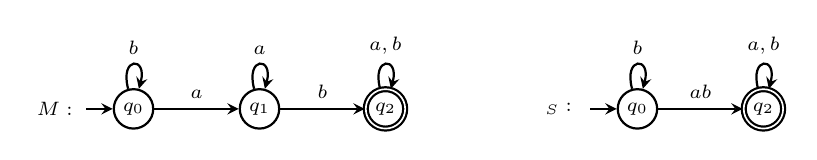
\begin{tikzpicture}[state/.style={circle, draw, thick, inner sep =
      2pt},scale=0.8]
    \begin{scope}[every node/.style={state}]
      \node (0) at (0,0) {\scriptsize $q_0$}; \node (1) at (2,0)
      {\scriptsize $q_1$}; \node [double] (2) at (4,0) {\scriptsize
        $q_2$};
    \end{scope}
    \begin{scope}[->, thick, >=stealth, auto]
      \draw (-0.75, 0) to (0); \draw (0) to node {\scriptsize $a$ }
      (1); \draw (1) to node {\scriptsize $b$} (2); \draw (0) to [loop
      above] node {\scriptsize $b$} (0); \draw (1) to [loop above]
      node {\scriptsize $a$} (1); \draw (2) to [loop above] node
      {\scriptsize $a,b$} (2);
    \end{scope}
    \node at (-1.25, 0) {\scriptsize $M:$};

    \begin{scope}[xshift=8cm]
      \begin{scope}[every node/.style={state}]
        \node (0) at (0,0) {\scriptsize $q_0$}; \node [double] (1) at
        (2,0) {\scriptsize $q_2$};
      \end{scope}
      \begin{scope}[->, thick, >=stealth, auto]
        \draw (-0.75, 0) to (0); \draw (0) to node {\scriptsize $ab$}
        (1); \draw (1) to [loop above] node {\scriptsize $a,b$} (1);
        \draw (0) to [loop above] node {\scriptsize $b$} (0);
      
      \end{scope}

      \node at (-1.25, 0) {\scriptsize $\Aa_S:$};
    \end{scope}
  \end{tikzpicture}
  \caption{DFA $M$ and an equivalent DSA $\Aa_S$ `induced' with
    $S = \{q_0, q_2\}$.}
  \label{fig:induced-eqv}
\end{figure}


\begin{figure}[t]
  \centering
  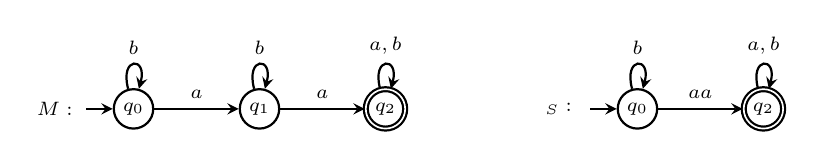
\begin{tikzpicture}[state/.style={circle, draw, thick, inner sep =
      2pt}, scale=0.8]
    \begin{scope}[every node/.style={state}]
      \node (0) at (0,0) {\scriptsize $q_0$}; \node (1) at (2,0)
      {\scriptsize $q_1$}; \node [double] (2) at (4,0) {\scriptsize
        $q_2$};
    \end{scope}
    \begin{scope}[->, thick, >=stealth, auto]
      \draw (-0.75, 0) to (0); \draw (0) to node {\scriptsize $a$ }
      (1); \draw (1) to node {\scriptsize $a$} (2); \draw (0) to [loop
      above] node {\scriptsize $b$} (0); \draw (1) to [loop above]
      node {\scriptsize $b$} (1); \draw (2) to [loop above] node
      {\scriptsize $a,b$} (2);
    \end{scope}
    \node at (-1.25, 0) {\scriptsize $M:$};

    \begin{scope}[xshift=8cm]
      \begin{scope}[every node/.style={state}]
        \node (0) at (0,0) {\scriptsize $q_0$}; \node [double] (1) at
        (2,0) {\scriptsize $q_2$};
      \end{scope}
      \begin{scope}[->, thick, >=stealth, auto]
        \draw (-0.75, 0) to (0); \draw (0) to node {\scriptsize $aa$}
        (1); \draw (1) to [loop above] node {\scriptsize $a,b$} (1);
        \draw (0) to [loop above] node {\scriptsize $b$} (0);
      
      \end{scope}

      \node at (-1.25, 0) {\scriptsize $\Aa_S:$};
    \end{scope}
  \end{tikzpicture}
  \caption{DFA $M$ and DSA $\Aa_S$ `induced' with $S = \{q_0,
    q_2\}$. Not equivalent.}
  \label{fig:induced-not-eqv}
\end{figure}






\begin{definition}[Simple words]\label{def:simple-words}
  Consider a complete DFA $M = (Q, \Sigma, q^{init}, \Delta, F)$. Let
  $S \incl Q$ be a subset of states, and $p, q \in Q$. We define
  $\spath{p}{q}{S}$, the \emph{simple words from $p$ to $q$ modulo
    $S$}, as the set of all words $a_1 a_2 \dots a_n \in \Sigma^+$
  such that there is a path:
  $p = p_0 \xra{a_1} p_1 \xra{a_2} \cdots p_{n-1} \xra{a_n} p_n = q$
  in $M$ where
  \begin{itemize}
  \item no intermediate state belongs to $S$:
    $\{ p_1, \dots, p_{n-1}\} \incl Q \setminus S$, and
  \item there is no intermediate cycle: if $p_i = p_j$ for some
    $0 \le i < j \le n$, then $p_i = p_0$ and $p_j = p_n$.
  \end{itemize}
  We write $\spaths{p}{S}$ for $\bigcup_{q \in Q} \spath{p}{q}{S}$,
  the set of all simple words modulo $S$, emanating from $p$.
\end{definition}

For example, in Figure~\ref{fig:induced-eqv}, with $S = \{q_0, q_2\}$,
we have $\spath{q_0}{q_1}{S} = \{a\}$, $\spath{q_0}{q_0}{S} = \{b\}$
and $\spath{q_0}{q_2}{S} = \{ab\}$. These are the same in
Figure~\ref{fig:induced-not-eqv}, except $\spath{q_0}{q_2}{S} = aa$.

Here are some preliminary technical lemmas.
Due to determinism of $M$, we get the following 
property, which underlies several arguments that come later.

\begin{lemma}
  Let $S \incl Q$, and $p, q, r \in Q$ s.t. $q \neq r$. We have
  $\spath{p}{q}{S} \cap \spath{p}{r}{S} = \emptyset$.
\end{lemma}

The next lemma says that every transition either extends a simple path
or is a ``back-edge'' leading to an ancestor in the path.

\begin{lemma}\label{lem:spaths-property}
  Let $S \incl Q$ and $p, q, u \in Q ~ (q \notin S, p \ne q) $ such
  that $q \xra{a} u$ is a transition. For every
  $\s \in \spath{p}{q}{S}$, either $\s a$ belongs to $\spath{p}{u}{S}$, or some
  proper prefix of $\s a$ belongs to $\spath{p}{u}{S}$.
\end{lemma}
\begin{proof}
  Since $\sigma \in \spath{p}{q}{S}$, there is a path
  $p = p_0 \xra{a_1} p_1 \xra{a_2} \cdots p_{n-1} \xra{a_n} p_n = q$,
  with $\s = a_1 a_2 \dots a_n$, satisfying the conditions of
  Definition~\ref{def:simple-words}. If $u \neq p_i$ for
  $0 \le i \le n$, then $\s a \in \spath{p}{u}{S}$ since $q \notin
  S$. If $u = p_i$ for some $0 < i \le n$, then the prefix
  $a_1 a_2 \dots a_{i-1} \in \spath{p}{u}{S}$. If $u = p_0$, then we
  have $\s a \in \spath{p}{u}{S}$.
\end{proof}


Fix a complete DFA $M$ for this section. A DSA can be `induced' from
$M$ using $S$, by fixing states to be $S$ (initial and final states
retained) and transitions to be the simple words modulo $S$ connecting
them i.e. $p \xra{\s} q$ if $\s \in \spath{p}{q}{S}$ (Figure
\ref{fig:induced-eqv}).

\begin{definition}[Induced DSA]\label{def:induced-dsa}
  Given a DFA $M$ and a set $S$ of states in $M$ that contains the
  initial and final states, we define the induced DSA of $M$ (using
  $S$). The states of the induced DSA are given by $S$. The initial
  and final states are the same as in $M$. The transitions are given
  by the simple words modulo $S$ i.e. $p \xra{\s} q$ if
  $\s \in \spath{p}{q}{S}$, for every pair of states $p, q \in S$.
\end{definition}

The induced DSA may not be language-equivalent (Figure
\ref{fig:induced-not-eqv}); to ensure that, we need to check some
conditions. Here is a central definition.

\begin{definition}[Suffix-compatible transitions]\label{def:suffix-compatibility}
  Fix a subset $S \incl Q$. A transition $q \xra{a} u$ is
  suffix-compatible w.r.t. $S$ if either
  $q \in S$ or $u \in S~\textbf{OR}$ for all $p \in S$, and for every
  $\s \in \spath{p}{q}{S}$, there is an $\a \in \spath{p}{u}{S}$ s.t.:
  \begin{itemize}
  \item $\a$ is a suffix of $\s a$, and
  \item moreover, $\a$ is the longest suffix of $\s a$ among words in
    $\spaths{p}{S}$.
  \end{itemize}
\end{definition}

Note that a transition $q \xra{a} u$ is trivially suffix-compatible if
$q \in S$ or $u \in S$. The rest of the condition only needs to be
checked when both of $q,u \notin S$. In
Figure~\ref{fig:induced-not-eqv}, we find the self-loop at $q_1$ to
not be suffix-compatible: we have $S = \{q_0, q_2\}$, and
$\spath{q_0}{q_1}{S} = \{ a \}$, $\spaths{q_0}{S} = \{b, a, ab\}$; the
transition $q_1 \xra{b} q_1$ is not suffix-compatible since there is
no suffix of $ab$ in $\spath{q_0}{q_1}{S}$. Whereas in
Figure~\ref{fig:induced-eqv}, the loop is labeled $a$ instead of
$b$. The transition $q_1 \xra{a} q_1$ is suffix-compatible, since the longest suffix of $aa$ among $\spaths{q_0}{S}$ is $a$ and it is
present in $\spath{q_0}{q_1}{S}$. Let us take the DFA in the right of
Figure~\ref{fig:dsa-to-dfa-eg}, and let $S = \{q, q'\}$. Here are some
of the simple path sets: $\spath{q}{ab}{S} = \{ab, bab, baab\}$,
$\spath{q}{aba}{S} = \{aba, baba, baaba\}$. Consider the transition
$aba \xra{b} ab$. It can be verified that for every
$\s \in \spath{q}{aba}{S}$, the longest suffix of the extension
$\s b$, among simple paths out of $q$, indeed lies in the state $ab$.
In fact, all transitions satisfy suffix-compatibility w.r.t. the
chosen set $S$.


The suffix-compatibility condition is described using simple paths to
states. It requires that every transition take each simple word
reaching its source to the state tracking the longest suffix of its
one-letter extension. This condition on simple paths, transfers to all
words, that circle around the suppressed states. In
Figure~\ref{fig:dsa-to-dfa-eg}, this property can be verified by
considering the word $bbabab$ and its run: $q \xra{b} b \xra{b} b \xra{a} ba \xra{b} ab \xra{a} aba \xra{b} ab$.
At each step, the state reached corresponds to the longest suffix
among the simple words out of $q$.
In the next two lemmas, we prove this claim.

We will use a special
notation: for a state $p \in S$, we write $\out(p, S)$ for
$\bigcup_{r \in S} \spath{p}{r}{S}$; these are the simple words that
start at $p$ and end in some state $r$ of $S$. Notice that these are
the words that appear as transitions in the induced DSA. In
particular, $\out(p)$ in the induced DSA equals $\out(p, S)$. We also remark that $\out(p,S)$ is different from $\spaths{p}{S}$: the latter considers simple words from $p$ to all states in $Q$, whereas the former only considers words from $p$ to $S$.


\begin{restatable}{lemma}{sfxCompatibleDfaToWords}
  \label{lem:sfx-compatibility-dfa-paths-to-words}
  Let $S$ be a set of states such that every transition of $M$ is
  suffix-compatible w.r.t. $S$. Pick $p \in S$, and let
  $w \in \Sigma^+$ be a word with a run
  $p = p_0 \xra{w_1} p_1 \xra{w_2} p_2 \dots p_{n-1} \xra{w_n} p_n$
  such that the intermediate states $p_1, \dots, p_{n-1}$ belong to
  $Q \setminus S$. The state $p_n$ may or may not be in $S$. Then:
  \begin{itemize}
  \item no proper prefix of $w$ has any word from $\out(p,S)$ as
    suffix (no factor of $w$ is in $\out(p,S)$), and
  \item there is $\a \in \spath{p}{p_n}{S}$ such that $\a$ is the
    longest suffix of $w$ among words in $\spaths{p}{S}$.
  \end{itemize}
\end{restatable}

\begin{proof}
  We prove this by induction on the length of the word $w$. When
  $w = a$ for $a \in \Sigma$, we have the run $p \xra{a} q$. The first
  conclusion of the lemma is vacuously true, since there is no
  non-empty proper prefix of $a$. For the second conclusion, note
  that, by definition, we have $a \in \spath{p}{q}{S}$ (in both cases
  when $q \neq p$ and $q = p$). Moreover, clearly $a$ is the longest
  suffix of $a$.

  Now, let $w = w'a$ with a run $p \xra{w'} p' \xra{a} p_n$ such that
  $p'$ and the intermediate states while reading $w'$ belong to
  $Q \setminus S$. Assume the lemma holds for $w'$.  Therefore, the
  longest suffix $\s'$ of $w'$, among $\spaths{p}{S}$, belongs to
  $\spath{p}{p'}{S}$, that is: $\s' \lsfx{\spaths{p}{S}} w'$ and
  $\s' \in \spath{p}{p'}{S}$ (notation as in
  Definition~\ref{def:notation}). We claim that the longest suffix of
  $w'a$ is in fact the longest suffix of $\s' a$.  If not: there
  is $\s'' a$ with $|\s''| > |\s'|$ such that
  $\s'' a \lsfx{\spaths{p}{S}} w' a$. Therefore
  $\s'' \lsfx{\spaths{p}{S}} w'$. This contradicts
  $\s' \lsfx{\spaths{p}{S}} w'$. If $p_n \in Q \setminus S$, the
  longest suffix of $\sigma' a$ lies in $p_n$, by suffix-compatibility
  (Definition~\ref{def:suffix-compatibility}). If $p_n \in S$, we will
  have the exact word $\s' a \in \spath{p}{p_n}{S}$. 
  
\end{proof}


\begin{restatable}{lemma}{sfxCompatibleWordsToDfa}
  \label{lem:sfx-compatibility-words-to-paths}
  Let $S$ be a set of states such that every transition of $M$ is
  suffix-compatible w.r.t. $S$. Let $p \in S$, and $w \in \Sigma^+$ be
  a word such that no proper prefix of $w$ has a word from
  $\out(p,S)$ as suffix (no factor of $w$ is in $\out(p,S)$). Then:
  \begin{itemize}
  \item The run of $M$ starting from $p$, is of the form
    $p \xra{w_1} p_1 \xra{w_2} p_2 \dots p_{n-1} \xra{w_n} p_n$ where
    $\{p_1, \dots, p_{n-1}\} \incl Q \setminus S$ (notice that we have
    not included $p_n$, which may or may not be in $S$).
  \item the longest suffix of $w$, among $\spaths{p}{S}$ lies in
    $\spath{p}{p_n}{S}$.
  \end{itemize}

\end{restatable}

\begin{proof}
  We prove this by induction on the length of the word $w$. Suppose
  $w = a$, for $a \in \Sigma$. Since $M$ is complete, there is a
  transition $p \xra{a} p_1$. The first item is vacuously
  true. Moreover, if there is $q \in S$ and $\a \in \spath{p}{q}{S}$
  such that $\a$ is a suffix of $a$, then clearly $\a = a$. Hence
  $q = p_1$, due to the determinism of the underlying automaton. If
  there is no such $q$, then it means $p_1\notin S$.

  Suppose $w = w'a$ satisfies the assumptions of the lemma. Assuming
  the lemma holds for $w'$, we have a run $p \xra{w'} p'$ such that
  $p'$ and all intermediate states lie in $Q \setminus S$. Let
  $p' \xra{a} p_n$ be the outgoing transition on $a$ from $p'$. This
  gives a path $p \xra{w'} p \xra{a} p_n$ satisfying the first part of
  the lemma. By the second item of
  Lemma~\ref{lem:sfx-compatibility-dfa-paths-to-words}, the longest
  suffix $\a'a$ of $w'a$ among $\spaths{p}{S}$ belongs to
  $\spath{p}{p_n}{S}$. % Therefore, if there is $q \in S$ as mentioned
  % in the second statement of the lemma, we require $q = p_n$ due to
  % determinism of the underlying automaton. Otherwise
  % $p_n \in Q \setminus S$. This concludes the proof in this case.
\end{proof}


Suffix-compatibility alone does not suffice to preserve the
language. In Figure~\ref{fig:well-formed-set}, consider
$S = \{0, 2, 4\}$. Every transition is suffix-compatible
w.r.t. $S$. The DSA induced using $S$ is shown in the middle. Notice
that it is not language equivalent, due to the word $aba$ for
instance. The run of $aba$ looks as follows: $0 \xra{ab} 4 \xra{b}
4$. The expected run was $0 \xra{aba} 2$, but that does not happen
since there is a shorter prefix with a matching transition. Even
though, we have suffix-compatibility, we need to ensure that there are
no ``conflicts'' between outgoing patterns. This leads to the next
definition.



\begin{definition}[Well-formed set]\label{def:well-formed-set}
  A set of states $S \incl Q$ is well-formed if there is no
  $p \in S, q \in S$ and $q' \notin S$, with a pair of words
  $\a \in \spath{p}{q}{S}$ (simple word to a state in $S$) and
  $\beta \in \spath{p}{q'}{S}$ (simple word to a state not in $S$)
  such that $\alpha$ is a suffix of $\beta$.
\end{definition}

We observe that the set $S=\{0,2,4\}$ is not well-formed since
$b \in \spath{0}{4}{S}, ab \in \spath{0}{3}{S}$ and $b$ is a suffix of
$ab$. Whereas $S'=\{0,2,3,4\}$ is both suffix-tracking, and
well-formed, and induces an equivalent DSA. On the word $aba$, the run
on the DSA would be $0 \xra{ab} 3 \xra{a} 2$. The first move
$0 \xra{ab} 3$ applies the longest match criterion, and fires the $ab$ transition
since $ab$ is a longer suffix than $b$.  This was not possible before
since $3 \notin S$. It turns out that the two conditions --- suffix-compatibility and
well-formedness --- are sufficient to induce a language equivalent
DSA.

\begin{figure}[t]
  \centering
  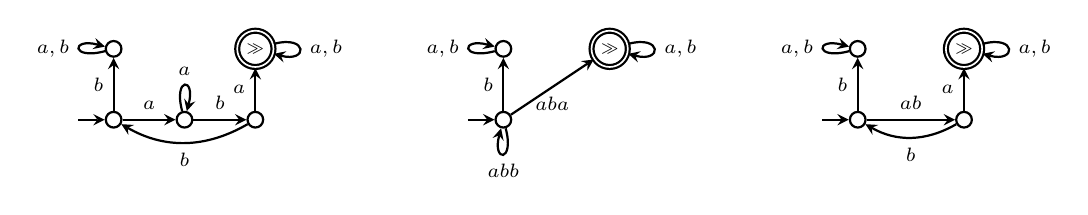
\begin{tikzpicture}[state/.style={circle, draw, thick, inner sep =
      2pt}, scale=0.9]
    \begin{scope}[every node/.style={state}]
      \node (0) at (-0.5,0) {\tiny $\rr$}; \node (1) at (0.5, 0)
      {\tiny $\bb$}; \node (2) at (1.5, 0) {\tiny $\yy$}; \node
      [double] (3) at (1.5, 1) {\tiny $\gg$}; \node (4) at (-0.5, 1)
      {\tiny $\ww$};
    \end{scope}
    \begin{scope}[->, thick, >=stealth, auto]
      \draw (-1, 0) to (0); \draw (0) to node {\scriptsize $a$} (1);
      \draw (0) to node {\scriptsize $b$} (4); \draw (1) to [loop
      above] node {\scriptsize $a$} (1); \draw (1) to node
      {\scriptsize $b$} (2); \draw (2) to node {\scriptsize $a$} (3);
      \draw (4) to [loop left] node {\scriptsize $a, b$} (4); \draw
      (3) to [loop right] node {\scriptsize $a, b$} (3); \draw (2) to
      [bend left=30] node {\scriptsize $b$} (0);
    \end{scope}

   
    \begin{scope}[xshift=5 cm]
      \begin{scope}[every node/.style={state}]
        \node (0) at (0,0) {\tiny $\rr$}; \node [ double] (3) at (1.5,
        1) {\tiny $\gg$}; \node (4) at (0, 1) {\tiny $\ww$};
      \end{scope}
      \begin{scope}[->, thick, >=stealth, auto]
        \draw (-0.5, 0) to (0); \draw (0) to node [below] {\scriptsize
          $aba$} (3); \draw (0) to node {\scriptsize $b$} (4); \draw
        (0) to [loop below] node {\scriptsize $abb$} (0); \draw (4) to
        [loop left] node {\scriptsize $a, b$} (4); \draw (3) to [loop
        right] node {\scriptsize $a, b$} (3);
      
      \end{scope}

    \end{scope}

   
    \begin{scope}[xshift=10cm]
      \begin{scope}[every node/.style={state}]
        \node (0) at (0,0) {\tiny $\rr$}; \node [double] (3) at (1.5,
        1) {\tiny $\gg$}; \node (2) at (1.5, 0) {\tiny $\yy$}; \node
        (4) at (0, 1) {\tiny $\ww$};
      \end{scope}
      \begin{scope}[->, thick, >=stealth, auto]
        \draw (-0.5, 0) to (0); \draw (0) to node {\scriptsize $ab$}
        (2); \draw (0) to node {\scriptsize $b$} (4); \draw (2) to
        node {\scriptsize $a$} (3); \draw (4) to [loop left] node
        {\scriptsize $a, b$} (4); \draw (3) to [loop right] node
        {\scriptsize $a, b$} (3); \draw (2) to [bend left=30] node
        {\scriptsize $b$} (0);
      \end{scope}

    \end{scope}
  \end{tikzpicture}
  \caption{A DFA, a non-equivalent DSA and an equivalent induced DSA. }
  \label{fig:well-formed-set}
\end{figure}



\begin{definition}[Suffix-tracking sets]\label{def:suffix-tracking-set}
  A set of states $S \incl Q$ is suffix-tracking if it contains the
  initial and accepting states, and
  \begin{enumerate}
  \item every transition of $M$ is suffix-compatible w.r.t. $S$,
  \item and $S$ is well-formed.
  \end{enumerate}
\end{definition}

All these notions lead to the main theorem of this section.

\begin{restatable}{theorem}{suffixTrackingCorrect}
  \label{thm:suffix-tracking-is-correct}
  Let $S$ be a suffix-tracking set of complete DFA $M$, and let
  $\Aa_S$ be the DSA induced using $S$. Then: $\Ll(\Aa_S) = \Ll(M)$
\end{restatable}
\begin{proof}
  Pick $w \in \Ll(M)$. There is an accepting run
  $q_0 \xra{w_1} q_1 \xra{w_2} \dots \xra{w_n} q_n$ of $M$ on $w$. By
  Definition~\ref{def:suffix-tracking-set}, we have $q_0, q_n \in
  S$. Let $1 \le i \le n$ be the smallest index greater than $0$, such
  that $q_i \in S$. Consider the run segment
  $q_0 \xra{w_1} q_1 \xra{w_2} \dots \xra{w_i} q_i$. By
  Lemma~\ref{lem:sfx-compatibility-dfa-paths-to-words}, and by the
  definition of induced DSA~\ref{def:induced-dsa}, no transition of
  $\Aa_S$ out of $q_0$ is triggered until $w_1 \dots w_{i-1}$, and
  then on reading $w_i$, the transition $q_0 \xra{\a} q_i$ is
  triggered, where $\a \in \spath{p}{q}{S}$, and $\a$ is also the
  longest suffix of $w_1 \dots w_i$ among $\spaths{p}{S}$. In
  particular, it is the longest suffix among outgoing labels from
  $q_0$ in $\Aa_S$. This shows there is a move
  $q_0 \xra[\a]{w_1 \dots w_i} q_i$ in $\Aa_S$. Repeat this argument
  on rest of the run
  $q_i \xra{w_{i+1}} q_{i+1} \xra{w_{i+1}} \dots \xra{w_n} q_n$ to
  extend the run of $\Aa_S$ on the rest of the word. This shows
  $w \in \Ll(\Aa_S)$.
  
  Pick $w \in \Ll(\Aa_S)$. There is an accepting run $\rho$ of $\Aa_S$
  starting at the initial state $q_0$. Consider the first move
  $q_0 \xra[\a]{w_1 \dots w_i} q_i$ of $\Aa_S$ on the word. By the
  semantics of a move (Definition~\ref{def:DSA-moves}) and
  Lemma~\ref{lem:sfx-compatibility-words-to-paths}, we obtain a run
  $q_0 \xra{w_1} q_1 \xra{w_2} \dots q_{i-1} \xra{w_i} q_i$ of $M$
  where the intermediate states $q_1, \dots, q_{i-1}$ lie in
  $Q \setminus S$. We apply this argument for each move $\rho$ in the
  accepting run of $\Aa_S$ to get an accepting run of $M$.
\end{proof}

We extend the idea of well-formed set of states to a corresponding notion on DSAs. We will employ this notion when we remove some unnecessary transitions from the induced DSAs that are obtained.

\begin{definition}[Well-formed DSA]\label{def:well-formed-dsa}
  A DSA $\Aa$ is \emph{well-formed} if for every state $q$, no
  outgoing label $\a \in \out(q)$ is a suffix of some proper prefix
  $\beta'$ of another outgoing label $\beta \in \out(q)$.
\end{definition}

\paragraph{Removing some redundant transitions.}
Let us now get back to Figure~\ref{fig:dsa-to-dfa-eg} to see if we can
derive the DSA on the left from the DFA on the right (assuming $q$ is
the initial state). As seen earlier, the set $S = \{q, q'\}$ is
suffix tracking. It is
also well formed since $baaa$ is not a suffix of any prefix of $abaa$
and vice-versa. The DSA $\Aa_S$ induced using $q$ and $q'$ will have
the set of words in $\spath{q}{q'}{S}$ as transitions between $q$ and
$q'$. Both $abaa$ and $baaa$ belong to $\spath{q}{q'}{S}$. However,
there are some additional simple words: for instance, $abbaaa$. Notice
that $baaa$ is a suffix of $abbaaa$, and therefore even if we remove the
transition on $abbaaa$, there will be a move to $q'$ via
$q \xra{baaa} q'$. This tempts us to use only the suffix-minimal words
in the transitions of the induced DSA. This is not always safe, as we
explain below. We show how to carefully remove
``bigger-suffix-transitions''.

Consider the DSA on the left in
Figure~\ref{fig:bigger-suffix-transitions}. If $caba$ is removed, the
moves which were using $caba$ can now be replaced by $ba$ and we still
have the same pair of source and target states. Consider the picture
on the right of the same figure. There is an outgoing edge to a
different state on $aba$. Suppose we remove $caba$. The word $caba$
would then be matched by the longer suffix $aba$ and move to a
different state.
Another kind of redundant transitions are some of the self-loops on
DSAs. In Figure~\ref{fig:induced-eqv}, the self-loop on $b$ at $q_0$
can be removed, without changing the language. This can be generalized
to loops over longer words, under some conditions. 



\begin{figure}[t]
  \centering
  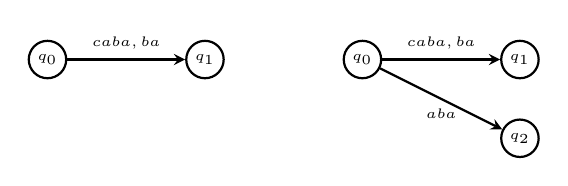
\begin{tikzpicture}[state/.style={circle, draw, thick, inner sep =
      2pt}]
    \begin{scope}[every node/.style={state}]
      \node (0) at (0,0) {\tiny $q_0$}; \node (1) at (2,0) {\tiny
        $q_1$};
    \end{scope}
    \begin{scope}[->, >=stealth, thick, auto]
      \draw (0) to node {\tiny $caba, ba$} (1);
    \end{scope}

    \begin{scope}[xshift=4cm]
      \begin{scope}[every node/.style={state}]
        \node (0) at (0,0) {\tiny $q_0$}; \node (1) at (2,0) {\tiny
          $q_1$}; \node (2) at (2,-1) {\tiny $q_2$};
      \end{scope}
      \begin{scope}[->, >=stealth, thick, auto]
        \draw (0) to node {\tiny $caba, ba$} (1); \draw (0) to node
        [below] {\tiny $aba$} (2);
      \end{scope}
    \end{scope}
  \end{tikzpicture}
  \caption{Illustrating bigger-suffix transitions and when they are
    redundant}
  \label{fig:bigger-suffix-transitions}
\end{figure}

\begin{definition}\label{def:redundant-transitions}
  Let $\Aa$ be a DSA, $q, q'$ be states of $\Aa$ and
  $t:= q \xra{\a} q'$ be a transition.

  We call $t$ a \emph{bigger-suffix-transition} if there exists
  another transition $(q, \beta, q')$ with $\beta$ a suffix of $\alpha$. 

  If there is a transition $t' := q \xra{\gamma} q'' ~ (q'' \neq q')$,
  such that $\beta$ is a suffix of $\gamma$, and $\gamma$ is a suffix
  of $\alpha$, we call $t$ \emph{useful}. A
  bigger-suffix-transition is called \emph{redundant} if it is not
  useful.

  We will say that $t$ is a \emph{redundant self-loop} if $q = q'$,
  $q$ is not an accepting state, and no suffix of $\a$ is a prefix of
  some outgoing label in $\out(q)$.
\end{definition}

In Figure~\ref{fig:bigger-suffix-transitions}, for the automaton on
the left, the transition on $caba$ is redundant. Whereas for the DSA on
the right, $caba$ is a bigger-suffix-transition, but it is
useful. The
self-loop on $q_0$ in Figure~\ref{fig:induced-eqv} is
redundant, but the loop on $q_0$ in Figure~\ref{fig:example-ab-bb}
is useful. Lemmas~\ref{lem:bigger-suffix-transitions-redundant}
and~\ref{lem:removable-self-loop-redundant} 
prove correctness of
removing redundant transitions.

\begin{lemma}
  \label{lem:bigger-suffix-transitions-redundant}
  Let $\Aa$ be a DSA, and let $t:= q \xra{\a} q'$ be a redundant
  bigger-suffix-transition. Let $\Aa'$ be the DSA obtained by removing
  $t$ from $\Aa$. Then, $L(\Aa) = L(\Aa')$.
\end{lemma}
\begin{proof} 
  
 \emph{To show $L(\Aa) \incl L(\Aa')$.} Let $w \in L(\Aa)$ and let
  $q_0 \xra[\a_0]{w_0} q_1 \xra[\a_1]{w_1} \cdots
  \xra[\a_{m-1}]{w_{m-1}} q_m$ be an accepting run. If no
  $(q_i, \a_i, q_{i+1})$ equals $(q, \a, q')$, then the same run is
  present in $S'$, and hence $w \in L(S')$. Suppose
  $(q_j, \a_j, q_{j+1}) = (q, \a, q')$ for some $j$. So, the word
  $w_{j}$ ends with $\a$. As $(q, \a, q')$ is a
  bigger-suffix-transition, there is another $(q, \beta, q')$ such that
  $\beta \sfx \a$. Therefore, the word $w_j$ also ends with $\beta$. Since
  there was no transition matching a proper prefix of $w_j$, the same
  will be true at $\Aa'$ as well, since it has fewer transitions. It
  remains to show that $q_j \xra[\beta]{w_j} q_{j+1}$ is a move. The only
  way this cannot happen is if there is a $q \xra{\gamma} q''$ with
  $\beta \sfx \gamma \sfx \a$. But this is not possible since
  $q \xra{\a} q'$ is a redundant bigger-suffix transition. Therefore,
  every move using $(q, \a, q')$ in $\Aa$ will now be replaced by
  $(q, \beta, q')$ in $\Aa'$. Hence we get an accepting run in $\Aa'$,
  implying $w \in L(\Aa')$.

  \emph{To show $L(\Aa') \incl L(\Aa)$}. Consider $w \in L(\Aa')$ and
  an accepting run
  $q_0 \xra[\a_0]{w_0} q_1 \xra[\a_1]{w_1} \cdots
  \xra[\a_{m-1}]{w_{m-1}} w_m$ in $\Aa'$. Notice that if
  $q \xra[\beta]{w_j} q'$ is a move in $\Aa'$, the same is a move in
  $\Aa$ when $\a \not\sfx w_j$. When $\a \sfx w_j$, then the
  bigger-suffix-transition $q \xra{\a} q'$ will match and the move $q
  \xra[\beta]{w_j} q'$ 
  gets replaced by $q \xra[\a]{w_j} q'$. Hence we will get the same
  run, except that some of the moves using $q \xra{\beta} q'$ may get
  replaced with $q \xra{\a} q'$.
\end{proof}

For the correctness of removing redundant self-loops, we assume that the
DFA that we obtain is well-formed
(Definition~\ref{def:well-formed-dsa}) and has no redundant
bigger-suffix-transitions. The induced DSA that we obtain from
suffix-tracking sets is indeed well-formed. Starting from this induced
DSA, we can first remove all redundant bigger-suffix-transitions, and
then remove the redundant self-loops.

\begin{lemma}
  \label{lem:removable-self-loop-redundant}
  Let $\Aa$ be a well-formed DSA that has no removable
  bigger-suffix-transitions. Let $t := (q, \a, q)$ be a removable
  self-loop. Then the DSA $\Aa'$ obtained by removing $t$ from $\Aa$
  satisfies $\Ll(\Aa) = \Ll(\Aa')$.
\end{lemma}
\begin{proof}
 \emph{To show $\Ll(\Aa) \incl \Ll(\Aa')$}. Let $w \in \Ll(\Aa)$ and
  let $\rho:= q_0 \xra{w_0} q_1 \xra{w_1} \cdots \xra{w_{m-1}} q_m$ be
  an accepting run. Suppose $t$ matches the segment
  $q_j \xra{w_j} q_{j+1}$. Hence $q_j = q_{j+1} = q$.  Observe that as
  $q$ is not accepting, we have $j+1 \neq m$. Therefore there is a
  segment $q_{j+1} \xra{w_{j+1}} q_{j+2}$ in the run. We claim that if
  $t$ is removed, then no transition out of $q$ can match any prefix
  of $w_j w_{j+1}$.

  First we see that no prefix of $w_j$ can be
  matched, including $w_j$ itself: if at all there is a match, it
  should be at $w_j$, and a $\beta$ that is smaller than $\a$. By
  assumption, $\a$ is not a removable
  bigger-suffix-transition. Therefore, there is a transition $q
  \xra{\gamma} q'$, with $\beta \sfx \gamma \sfx \alpha$. This
  contradicts the assumption that $\alpha$ is a removable
  self-loop. Therefore there is no match upto $w_j$.

  Suppose some $(q, \beta, q')$
  matches a prefix $w_j u$ such that $\beta = v u$, that is, $\beta$
  overlaps both $w_j$ and $w_{j+1}$. If $\a \sfx v$, then it violates
  well-formedness of $S$ since it would be a suffix of a proper prefix
  ($v$) of $\beta$. This shows $v \sfx \a$ (since both are suffixes of
  $w_j$) and $v \prfx \beta$, contradicting the assumption that $t$ is
  removable. Therefore, $\beta$ does not overlap $w_j$. But then, if $\beta$
  is a suffix of a proper prefix of $w_{j+1}$, we would not have the
  segment $q_{j+1} \xra{w_{j+1}} q_{j+2}$ in the run
  $\rho$. Therefore, the only possibility is that we have a segment
  $q_j \xra{w_j w_{j+1}} q_{j+2}$. We have fewer occurrences of the
  removable loop $(q, \a, q)$ in the modified run. Repeating this
  argument for every match of $(q, \a, q)$ gives an accepting run of
  $\Aa'$. Hence $w \in L(\Aa')$.

  \emph{To show $L(\Aa') \incl L(\Aa)$.} Let $w \in L(\Aa')$ and
  $\rho' := q_0 \xra{w_0} q_1 \xra{w_1} \cdots \xra{w_{m-1}} q_m$ be
  an accepting run in $\Aa'$. Suppose $q_j \xra{w_j} q_{j+1}$ is
  matched by $(q, \beta, q')$. Let $w_j = v u $ with $\a \sfx v$. Then
  the removable-self-loop $(q, \a, q)$ will match the prefix
  $v$. Suppose $\beta$ overlaps with both $v$ and $u$, that is $\beta
  = \beta' u$. We cannot have $\alpha \sfx \beta'$ due to
  well-formedness of $\Aa$. We cannot have $\beta' \sfx \alpha$ since
  this would mean there is a suffix of $\alpha$ which is a prefix of $\beta$,
  violating the removable-self-loop condition.  Therefore,
  $\beta$ is entirely inside $u$, that is, $\beta \sfx
  u$. Hence in $\Aa$ the run will first start with $q \xra{v}
  q$. Applying the same
  argument, prefixes of the remaining word where 
  $t$ matches will be matched until there is a part of the word where
  $(q, \beta, q')$ matches. This applies to every segment, thereby giving
  us a run in $\Aa$.
\end{proof}


We now get to the core definition of this section, which tells how to
derive a DSA from a DFA, using the methods developed so far.

\begin{definition}[DFA-to-DSA derivation] \label{def:derived-dsa}
  A DSA is said to be \emph{derived from} DFA $M$ using
  $S \subseteq Q$, if it is identical to an induced DSA of $M$
  (using $S$) with all redundant transitions removed.
\end{definition}

By Theorem~\ref{thm:suffix-tracking-is-correct} and Lemma
\ref{lem:bigger-suffix-transitions-redundant}, we get the following
result.

\begin{theorem}
  Every DSA that is derived from a complete DFA using a suffix-tracking set, is language equivalent
  to it.
\end{theorem}


%%% Local Variables:
%%% mode: latex
%%% TeX-master: "dsa-main"
%%% End:


This chapter has provided a concrete answer to the constructive question that concluded the previous one: how to build a DSA for a given regular language. We have developed a complete and sound derivation procedure that transforms a given complete DFA into a language-equivalent DSA, providing the crucial bridge from the theoretical model to its practical application.

The core of this method is the concept of the \textit{suffix-tracking set}. By identifying the key technical conditions of \textit{suffix-compatibility}, which ensures the internal consistency of the suppressed automaton paths, and \textit{well-formedness}, which ensures non-ambiguous connections at the path endpoints, we established a rigorous framework for abstracting away DFA states while correctly preserving the original language's semantics within the suffix-reading paradigm. The procedure is fully constructive, providing a clear algorithm for generating correct DSAs, complete with post-processing steps to prune redundant transitions for improved conciseness.

Having established a method for constructing correct DSAs, the focus naturally shifts to optimization. Our procedure allows for many possible suffix-tracking sets within a single DFA, each yielding a different DSA of potentially different size. This raises the fundamental question of \textbf{minimization}: how can we find a DSA with the smallest possible total size for a given language? One might intuitively expect that applying our derivation procedure to the canonical (minimal-state) DFA would be the optimal strategy, mirroring the approach for models like DGAs~\cite{giammarresi1999deterministic}. The next chapter will investigate this question and reveal a surprising departure from this classical principle. We will explore the counter-intuitive landscape of DSA minimization, demonstrating that the path to an optimal DSA is fraught with complexities and that the canonical DFA is not always the best starting point.